\subsection{Trigger Selection}
\label{sect:triggerselection}
To investigate the efficiency of different trigger sets the SMST2tt sample is used. The selection cuts described in section \ref{subsect:mt2bcuts} are applied on top of the trigger selection. The ratio of the signal events passing all the cuts is shown for two different sets of triggers as a function of $\tilde{t}$ mass and $\tilde{\chi^0_1}$ mass in figure \ref{fig:trg_eff}. Although the signal efficiency is $\sim 4$ times larger when the $HT$ trigger is used, MC studies show that the number of remaining backgrounds are so larger that the multi-jet trigger is more powerful to exclude. The estimated exclusion power of both triggers are compared in figure \ref{fig:trgs_exclusion_powers}.

\begin{figure}[htbp] 
\centering
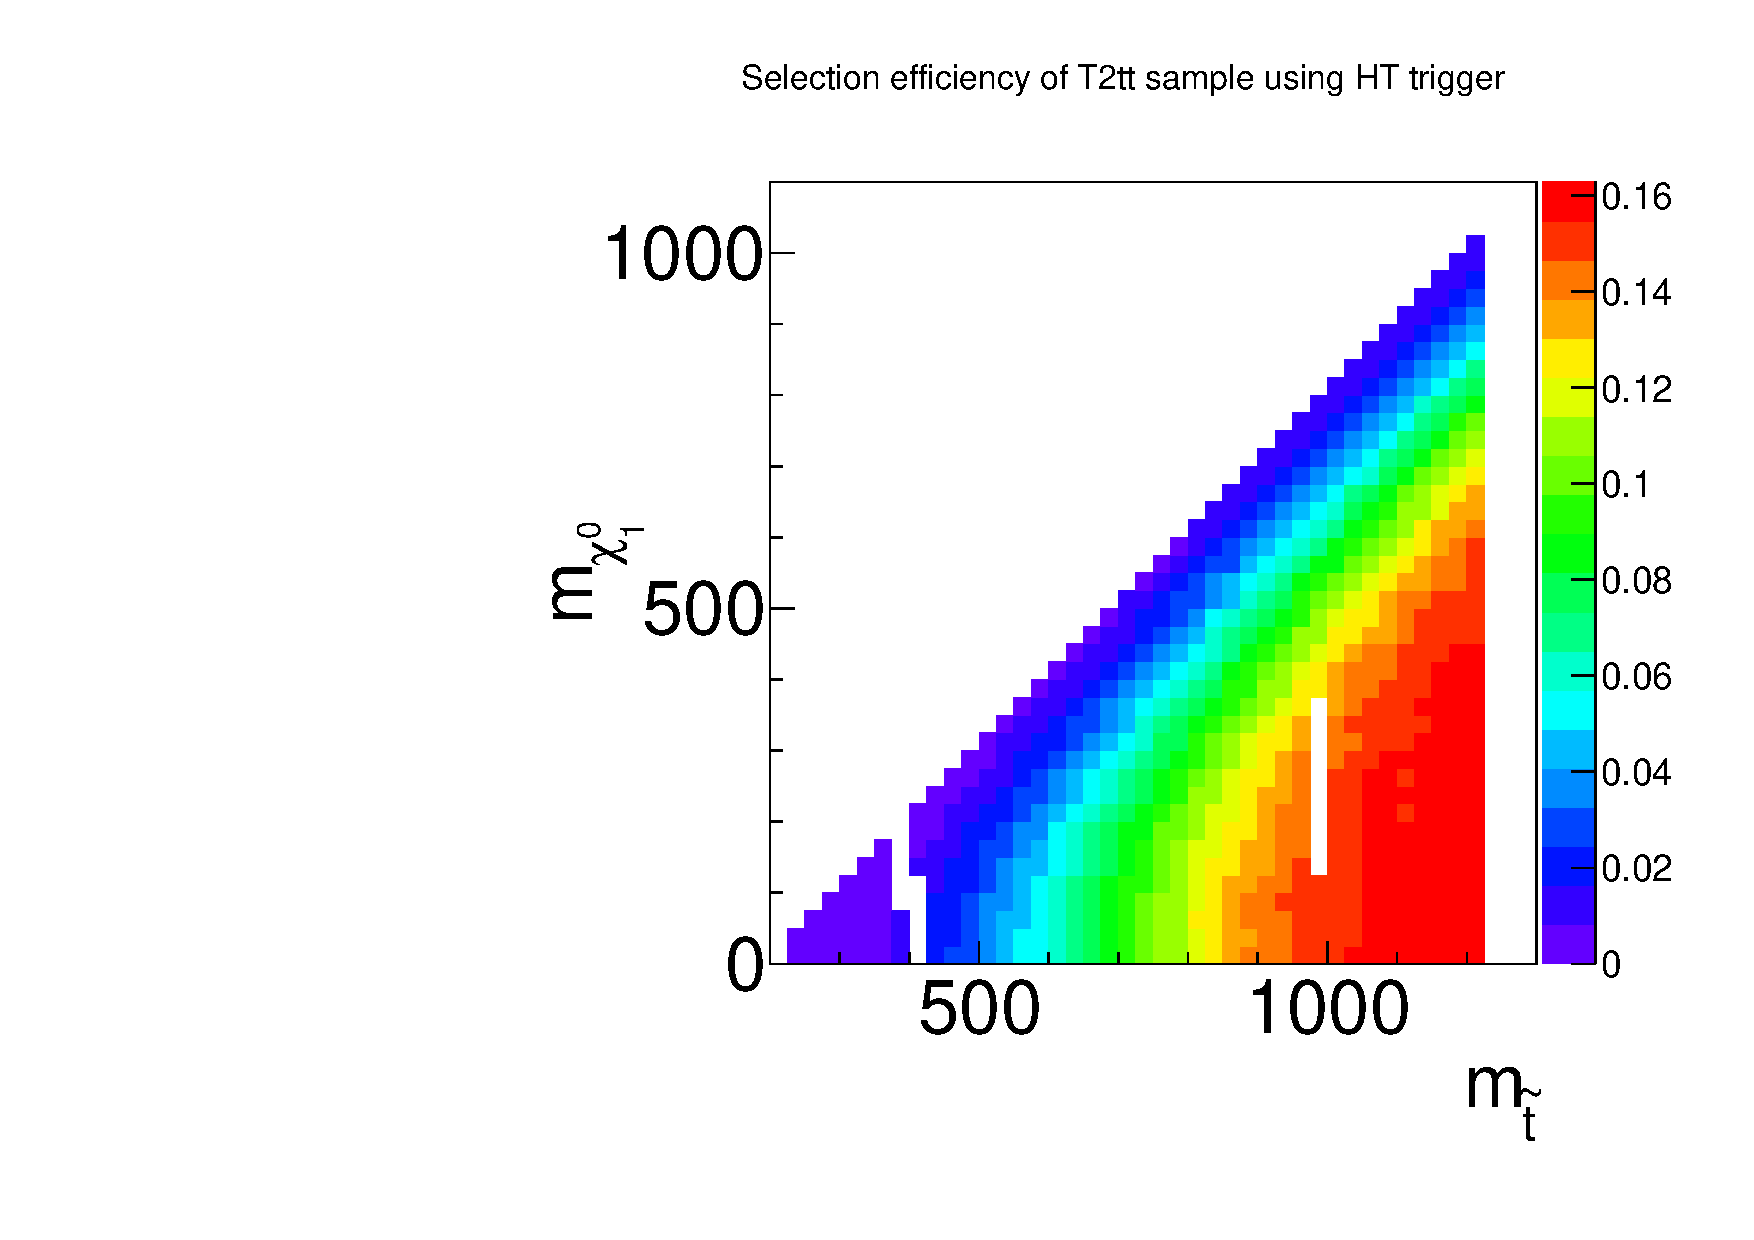
\includegraphics[angle=0,scale=0.39]{figs/HT_eff.pdf}
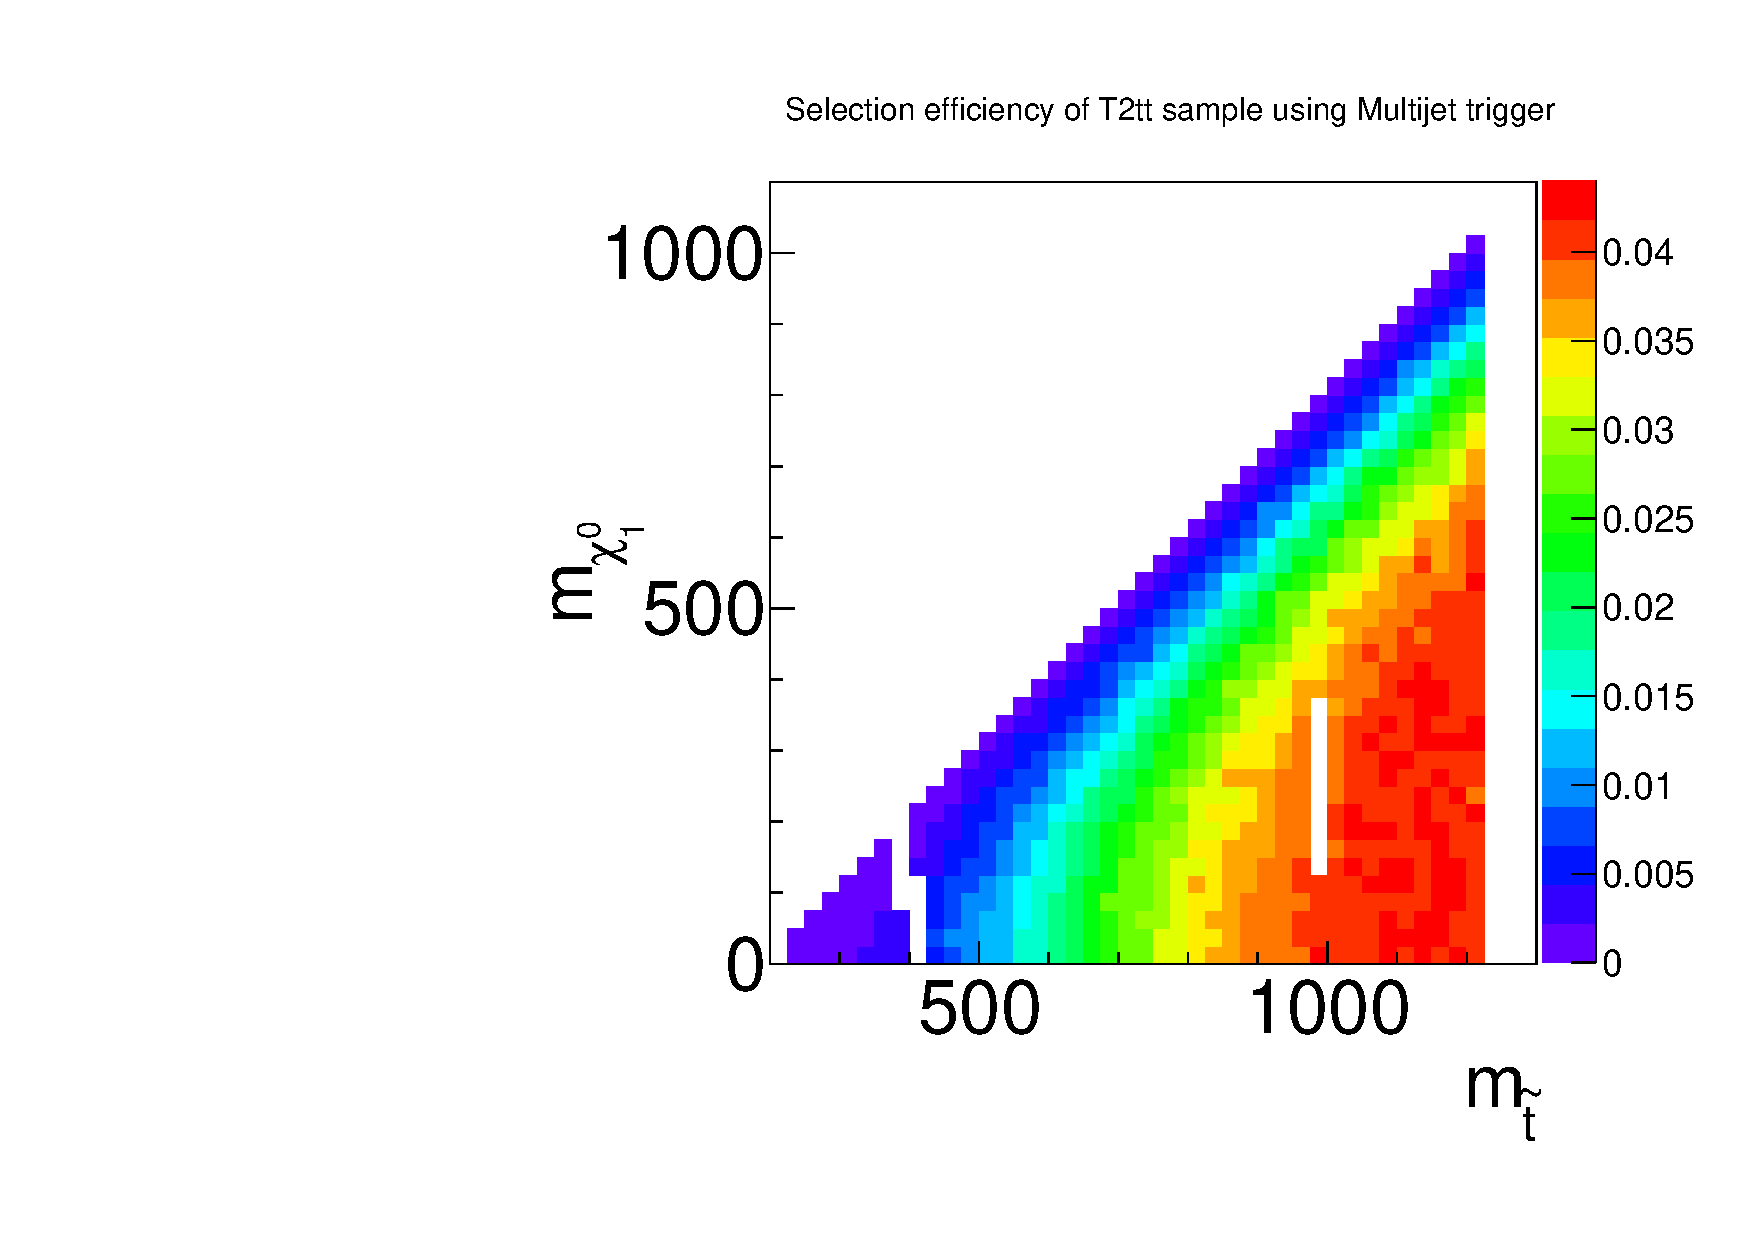
\includegraphics[angle=0,scale=0.39]{figs/multijet_eff.pdf} \\
\caption{The efficiency of different trigger sets (Left : HT trigger, Right : Multijet trigger) for the SMST2tt sample. The results are shown as a function of the $\tilde{t}$ mass and $\tilde{\chi^0_1}$ mass.}
\label{fig:trg_eff}
\end{figure}

\begin{figure}[htbp] 
\centering
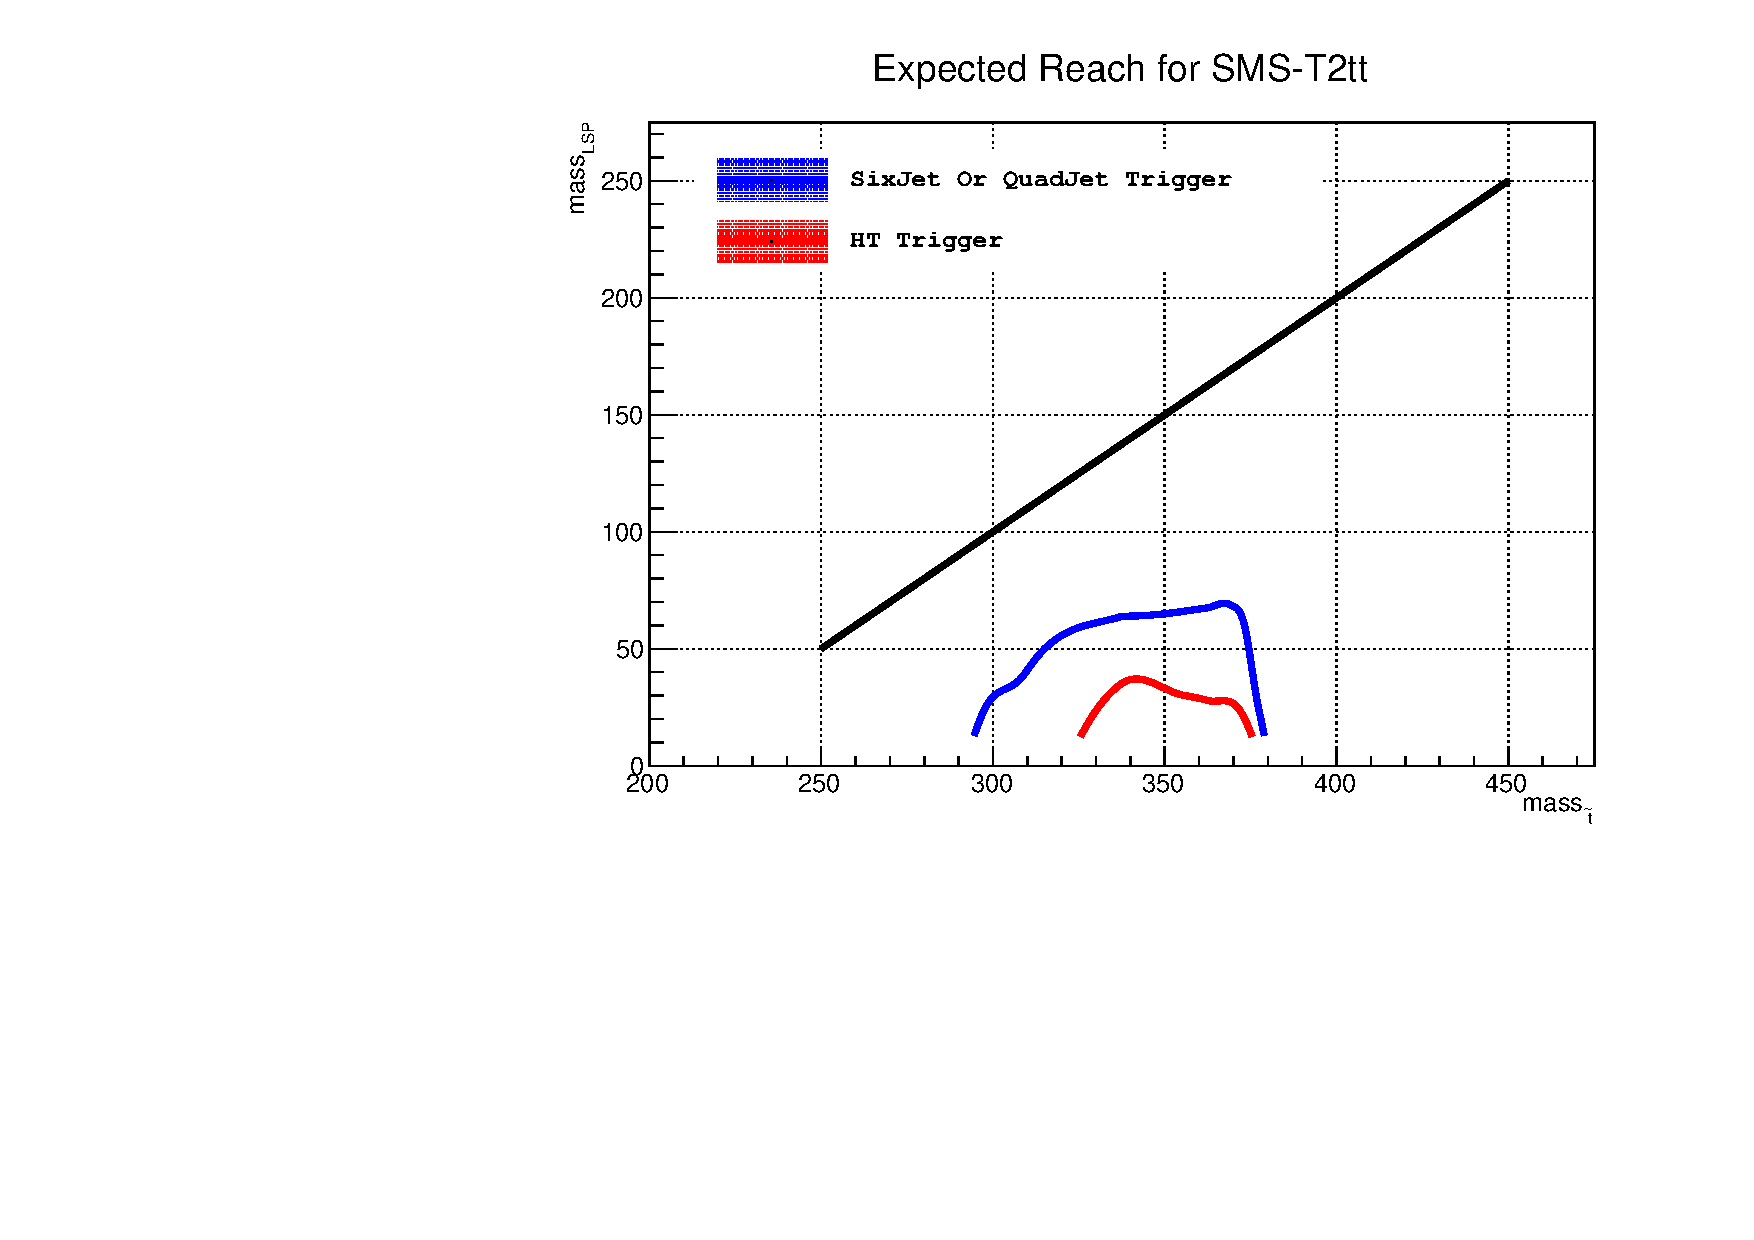
\includegraphics[angle=0,scale=0.5]{figs/SMST2tt_20121114.pdf}
\caption{The estimated exclusion power for two different sets of triggers. The multijet trigger is used in this analysis.}
\label{fig:trgs_exclusion_powers}
\end{figure}
The multi-jet trigger is used in the rest of the analysis.